\documentclass[12pt, a4paper, openany]{report}
\usepackage[left=3cm,top=3cm, bottom=3cm, right=4cm]{geometry}

% my custom stlye and functions stuff
\usepackage{mystyle}
\usepackage{csquotes}

\pagestyle{fancy}
\fancyhf{}
\lhead{Jan van Dick}
\chead{\glqq Zweite Natur und Befreiung\grqq}
\rhead{\thepage}

\title{
    {Zwischen Kritik und Affirmation}\\ 
    {\large- Zweite Natur und Befreiung bei Hegel und Nietzsche}\\
    {\large(Between Critique and Affirmation - Second Nation and Liberation in the Philosophies of Hegel and Nietzsche)}\\
    {\bigskip}
    {\large Goethe Universität Frankfurt am Main}\\
    {\bigskip}    
    {\bigskip}    
    {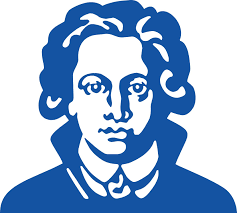
\includegraphics{logo.png}}\\
    {\bigskip}    
    {Sommersemester 2020}\\
}
\author{
    {Jan van Dick}\\
    {6081227}
}
\date{\today}

\begin{document}

\maketitle
\frontmatter


\chapter*{Abstrakt} \todo[noline]{Ist das Abstrakt so sinnvoll?}
Friedrich Nietzsches These vom Tode Gottes aus \textit{Die Fröhliche Wissenschaft}, dass \glqq wir\grqq{} ihn getötet haben, ist mehr als bloße Negativität. 
Müsste der Mensch nicht selbst Gott werden, um ihn getötet zu haben?.\footcite[Vgl.][481]{nietzsche_morgenrote_1999} 
Und der Mensch ist Gott dadurch geworden, dass er ihn \textit{geschaffen} hat, dadurch nur konnte er ihn töten. 
In dem Tod Gottes, liegt, dass Gott selbst vom Menschen gesetzt, dass er Schein ist, der sich gegen ihn verselbstständigte.
Gott ist somit geistiges Produkt des Menschen, in dem der Geist selbst wieder zur Natur sich verkehrte.
Der Tod Gottes ist die Befreiung daraus.
Der \glqq Tolle Mensch\grqq{} erklärt aber zugleich, dass nur die wenigsten von dieser Tat wissen. 
Für die Einen ist der Tod Gottes, eine untergegangene Sonne, die Befreiung also wieder eine In-Natur-Verkehrtheit.
Nur für uns \glqq geborene Räthselrather\grqq, die den Tod Gottes im vollen Umfang begreifen, ist er ein \glqq neues offenes Meer\grqq\footcite[][573]{nietzsche_morgenrote_1999}.
Ist nun der Tod Gottes, die Befreiung aus der von ihm gesetzten Natur, das unbekannte, neue, offene, noch nie so offen gewesene Meer, oder ist er der Beginn des Wieder-in-Natur-Verkehrt-Seins, wie Christoph Menke es in der Analyse Hegels Begriffs der zweiten Natur beschreibt?\footcite[Vgl.][144]{menke_autonomie_2018}\\
Befreiung steht also zwischen Kritik (wieder-in-Natur-Verkehrtheit) und Affirmation (Einheit von Setzen und Sein).
Während Menke (und Hegel) Befreiung aus der zweiten Natur, nicht ohne eine neu hervorgebrachte zweite Natur, in welcher der Geist wieder in Natur verfällt lesen, erörtere ich die Frage, ob es in dem Motiv des \glqq neuen offenen Meeres\grqq{} und der \glqq geborenen Räthselrather\grqq{} bei Nietzsche, eine Befreiung aus der fortwährenden In-Natur-Verkehrtheit geben kann.
Es ist die Frage nach einer dritten Befreiung neben der Befreiung aus der 1. und der 2. Natur. 
Die Antwort dazu wird sich in der Arbeit als Ergebnis des Unterschiedes der \glqq Erkennenden\grqq{} bei Nietzsche geben:
Zwar kann Befreiung aus der Natur nicht ohne Setzen einer zweiten Natur geschehen, aber die Befreiung, die sich in dem Bewusstsein ihrer eigenen Kritik vollzieht, ist zugleich über ihrer eigene Befreiung hinaus.
Die dritte Befreiung ist damit allerdings keine Befreiung aus der Befreiung.
Befreiung bleibt notwendig: der Mensch kann Freiheit nicht \textit{haben}, er muss sie immer wieder selbst hervorbringen.


\tableofcontents

\mainmatter

\chapter{Einleitung}
So, wie Friedrich Nietzsche in dem Aphorismus vom \glqq Tollen Menschen\grqq{} in \textit{Die fröhliche Wissenschaft} die These vom Tode Gottes entfaltet, enthält sie weit mehr als die bloße Negation Gottes;
in ihr steckt eine dialektische Konzeption der Begriffe (zweite) Natur und Befreiung.\footcite[Vgl.][481]{nietzsche_morgenrote_1999}
Diese beiden Begriffe möchte ich aus der Sicht Nietzsches, sowie der von Christoph Menke rekonstruierten Perspektive Hegels untersuchen.
Beide Begriffe entfalten sich in ihrem Doppelcharakter: zweite Natur als Kritik und Affirmation, Befreiung als Macht und Ohnmacht des Geistes.
In der zweiten Natur schlägt Setzen in Sein um; hierin liegt zum Einen die Verwirklichung des Geistes (Affirmation), zum Anderen die In-Natur-Verkehrtheit, der Tod des Geistes durch den Geist (Kritik).\footcite[Vgl.][145]{menke_autonomie_2018}
Ebenso verhält es sich mit dem Begriff der Befreiung: 
sie ist 1. die \textit{Macht} des Geistes neues Hervorzubringen und die scheinbare Notwendigkeit des Bestehenden zu durchbrechen, 
2. aber die \textit{Ohnmacht} des Geistes, da die Befreiung nie abgeschlossen ist; die Macht der Befreiung ist die Schaffung einer \glqq neuen\grqq{} zweiten Natur, aus der der Geist sich befreite und nun erneut befreien muss.\footcite[Vgl.][80]{menke_autonomie_2018}\\
Doch während in Hegels Deutung der Geist in der Befreiung aus der zweiten Natur, auf Grund der Endlichkeit des menschlichen Geistes, wieder in Natur verfällt, scheint bei Nietzsche in der Metapher des neuen, offenen Meeres, die Perspektive die ewige Wiederholung der In-Natur-Verkehrtheit zu überwinden, gegeben zu sein.
Zugleich betonen sowohl Hegel, als auch Nietzsche Freiheit als nicht-gegeben: 
Freiheit wird bei beiden so gedacht, dass man sie \glqq nicht nur hat, sondern auch beständig  noch erwirbt und erwerben muss\grqq\footcite[][637]{nietzsche_morgenrote_1999}. 
Freiheit ist die Befreiung aus der jeweiligen Unfreiheit.\footcite[Vgl][227]{adorno_negative_dialektik_2003}\todo[noline]{Eingehen auf Geist = sich von Natur unterscheiden?} \\ 
Die Dialektik zwischen Freiheit und Notwendigkeit, Geist und Mechanismus, Endlichkeit und Unendlichkeit des Geistes, ist demnach Gegenstand meiner Arbeit. 
Die Leitfrage der Arbeit also: \textit{gibt es in Nietzsches Philosophie eine Möglichkeit der Überwindung der Notwendig-in-Natur-Verkehrtheit des Geistes?}\\
Aus der Position des oben erwähnten \glqq Tollen Menschen\grqq{} liegt es nahe, diese Möglichkeit in dem \textit{Vollzug} der Befreiung zu denken. 
Genauer: in einer Form des Bewusstseins in der Tätigkeit der Befreiung; 
eine Befreiung, die sich im Bewusstsein ihrer eigenen Kritik vollzieht.
Zugleich, muss aber der Schein selbst, \glqq mich fühlen lassen, dass hier Schein [...] und nichts mehr ist\grqq\footcite[][417.]{nietzsche_morgenrote_1999}.
Zu fragen wäre demnach, ob dieses Bewusst-Werden eine Arbeit des einzelnen Individuums ist, oder ob es aus der Struktur des Allgemeinen, aus der zweiten Natur, dem Schein selbst, hervorgehen kann.\\

Nietzsche Aussage über den Tod Gottes bedeutet nach der Form-Seite die Überwindung der vom Menschen gesetzten zweiten Natur (Gott), der inhaltlichen Seite nach aber, dass der Mensch Gott nicht mehr nötig hat und die Bestimmung des Gesetzes sich aus dem Menschen selbst entwickelt. 
Um also den Begriff der zweiten Natur zu erarbeiten, werde ich kurz auf den Begriff der Autonomie eingehen, da hier der Versuch, Gesetz und Freiheit zusammen und von Gott gelöst zu denken, seinen Ursprung nimmt. 
Der Begriff der zweiten Natur ergibt sich dann aus Hegels Kritik an Kants Autonomiebegriff.
%versucht Kant zwar mit dem kategorischen Imperativ aus dem Paradox der Autonomie zu entkommen, argumentiert Hegel, dass er sich hier in der Inhaltslosigkeit des Gesetzes wiederholt.
Hegels Ausweg besteht darin Freiheit sozial zu verstehen. 
Aus dieser Perspektive werde ich Hegels Begriff der Sittlichkeit als soziale Teilhabe entwickeln.
Doch auch hier wird sich das Paradox der Autonomie in der Begriff der Gewohnheit wiederholen.
Aus der erneuten Wiederholung des Paradox werde ich Hegels Begriff der Befreiung entwickeln.
Darin ergibt sich, wie oben angegeben, die Grenze des von Menke erarbeiteten Begriffs der Befreiung:
Macht und Ohnmacht der Befreiung: Freiheit und Unfreiheit bleiben untrennbar miteinander verbunden.
Durch die Hinzunahme Nietzsches, soll versucht werden über diese Grenze hinauszugehen.\\

\todo[noline]{This part and the next seam to say more or less the same}
Zunächst soll der Begriff der zweiten Natur aus der Perspektive Hegels erläutert werden. 
In einem \hyperref[abschnitt_1]{ersten Schritt} soll demnach der Hegelsche Begriff der zweiten Natur anhand von folgendem Zitat Menkes rekonstruiert werden:
\begin{itemize}
    \item[] Die Gewohnheit als zweite Natur [ist] geistig oder frei [...], insofern sie ein Ausdruck des Wollens (oder ein Setzen) ist, und [...] mechanisch oder unfrei [...], weil sie, einmal gesetzt, selbstständig und unbewusst wirkend ist.\footcite[][145]{menke_autonomie_2018}
\end{itemize}
Die Struktur des ersten Teils ergibt sich aus den zu klärenden Begriffen. 
Zuerst soll der Begriff der Gewohnheit aus der Sittlichkeit, als Schritt über den \glqq bloß moralischen Standpunkt[]\grqq\footcite[][§ 135, S.139]{hegel_grundlinien_2017} hinaus, erläutert werden (a). 
Daraus ergibt sich der Begriff des \glqq geistigen Mechanismus\grqq, in welchem die Gewohnheit sich als \glqq geistig oder frei\grqq{} und \glqq mechanisch oder unfrei\grqq{} ergibt.\footcite[][145]{menke_autonomie_2018} (b).
Schließlich soll der Begriff der zweiten Natur aus Hegels Perspektive, seinen Abschluss finden in der Dialektik zwischen endlichem und unendlichem Geist und dem Doppelcharakter der zweiten Natur als Kritik und Affirmation (c).\\
In einem \hyperref[abschnitt_2]{zweiten Schritt} soll gezeigt werden, dass bei Nietzsche ein ähnlicher Begriff der zweiten Natur aufgezeigt werden kann.\footnote{Ich halte diesen Schritt unter anderem des deshalb für sinnvoll, weil er rechtfertigt, warum ich meine, mit Nietzsche überhaupt über Menkes Begriff der Befreiung hinausgehen zu können.}
\todo[noline]{Generell mehr Begründung, wieso Nietzsche?}
Dabei soll bereits auf die Beantwortung der Leitfrage vorbereitet werden.
Zunächst soll der Begriff der zweiten Natur anhand von Nietzsches Begriff des \textit{Scheins} erläutert werden (a).
Die Befreiung aus dem (sog.) Schein wird darauffolgend in der Unterscheidung des Schauspielers und der Rolle aufgegriffen (b). 
Abschließend sollen beide Begriffe nochmals in dem Absatz über den tollen Menschen analysiert und zusammengebracht werden (c).
In der Darlegung Nietzsches Position wird der Begriff \glqq Bewusstsein der Scheinhaftigkeit\grqq{} bereits eine wichtige Rolle einnehmen und dient der späteren Beantwortung der Leitfrage.\\
Im \hyperref[abschnitt_3]{dritten Abschnitt} soll die Befreiung aus der zweiten Natur erläutert werden, da diese, im Vergleich zur Befreiung aus der ersten Natur bei Hegel und Menke, und letztendlich auch bei Nietzsche, uneindeutig bleibt.
Wie Befreiung aus der zweiten Natur überhaupt möglich ist und wie diese sich konkret vollzieht, ist notwendig, um zu diskutieren wie über diese hinausgegangen werden kann.\\
Im vierten und \hyperref[abschnitt_4]{letzten Schritt} soll es abschließend zu einer Diskussion und Beantwortung der Leitfrage kommen. 


\chapter{Hauptteil}
Um nochmals einen anderen Einstieg zu wählen und die Fragestellung, sowie den groben Umriss der Arbeit auf alternative Art und Weise darzustellen, und die Problematik gewissermaßen von hinten aufzurollen, sei hier ein Zitat Nietzsches vorangestellt, auf welches ich gegen Ende erneut eingehen werde:
\begin{itemize}
    \item[] \textelp{} so finden wir als reifste Frucht an ihrem [der Sittlichkeit] Baum das \so{souveraine} [sic] \so{Individuum}, das nur sich selbst gleiche, das von der Sittlichkeit der Sitte wieder losgekommene, das autonome übersittliche Individuum (denn \qq{autonom} und \qq{sittlich} schliesst sich aus) \textelp{} \footcite[][293]{nietzsche_jenseits_2014}
\end{itemize} 
Hier befinden sich verschiedene Konzepte und Probleme im Begriff der Freiheit und im Geist-Natur-Verhältnis, die in der folgenden Arbeit eine zentrale Rolle spielen. 
Diese sollen als Einleitung der Auseinandersetzung mit den Begriffen \emph{Befreiung} und \emph{zweite Natur} vorangehen.\\

\emph{1. Geist als aus der Natur hervorgehend und sich von ihr unterscheidend.}\\
Zunächst spricht Nietzsche im selben Abschnitt von der Sittlichkeit als eine \qq{\so{vorhistorische} Arbeit}\footcite[][293]{nietzsche_jenseits_2014}.
Diese Sittlichkeit beschreibt Nietzsche als die Entwicklung des Menschen, in der er sich durch Zurichtung und Gewohnheit von seiner Natur befreit, die aber zugleich der Freiheit gegenübersteht, weil sie eine neue Form von inneren Zwang, von innerer Notwendigkeit schafft (\qq{der Mensch [muss] \textelp{} \emph{notwendig} geworden sein}\footcite[][292]{nietzsche_jenseits_2014}).
Darum ist die \qq{reifste Frucht} der Sittlichkeit dasjenige Individuum, welches sich von ihr wieder befreit.
Ohne hier den Anspruch zu erheben, Nietzsche habe es genau so gemeint, oder sei selber Hegelianer, liegt hier dennoch etwas vor, was stark an Hegels Begriff des Geistes erinnert, nämlich, dass er dadurch bestimmt ist \qq{aus der Natur herzukommen und sich von der Natur zu befreien}\footcite[][294]{khurana_freiheit_2017}.%
\todo[noline]{Search for exact citation: \qq{Geist is wesentlich die [...]}}
\todo[noline]{About my reading of Nietzsche}
Dies bedeutet, dass der Geist nicht einmal aus der Natur hervorgegangen ist, sondern es immer wieder und immer wieder auch in den höheren Stufen des Geistes tut.
Wenn der Geist, wie Hegel sagt, wesentlich die Bewegung seiner Befreiung aus der Natur ist, dann ist die Frage, \emph{welche} Natur es ist, aus der er sich immer wieder befreit. 
Es ergibt sich daraus, das der Geist selbst, durch diese Bestimmung zur Natur zurückgeführt wird und dass die Natur, aus der er sich befreit, letztendlich eine Natur ist, die er sich selbst voraussetzt: zweite Natur.\footcite[Vgl.][320]{khurana_freiheit_2017}
Das meint Nietzsches Rede vom Vorhistorischen: 
der Geist hat sich von der Natur befreit, indem er die Sittlichkeit, seine eigene Natur gesetzt hat. 
Das Nicht-Mehr-Vorhistorische ist, sich auch von dieser wieder zu befreien.
Dadurch hat Freiheit auch bei Nietzsche explizit prozesshaften Charakter. 
Wie in der Einleitung bereits angedeutet, liegt hier auch die Leitfrage meiner Arbeit: \emph{inwiefern kann dieser Prozess aufhören und zu einem Ende kommen?}
Nietzsche spricht diesen Ausweg ganz konkret an, er spricht vom \qq{Ende des ungeheuren Prozesses} und vom \qq{übersittliche[n] Individuum}, welches an dessen Ende steht.\footcite[][293]{nietzsche_jenseits_2014} 
Aber ist dieses Ende auch bei Nietzsche schließlich so zu verstehen, dass kein Prozess mehr stattfindet und der übersittliche Menschen, seine Autonomie \emph{hat}?
Diese Frage soll am Ende der Arbeit beantwortet werden.\\

\emph{2. Sittlichkeit als Kontrast zur Autonomie}\\
Meine Arbeit wird von dem Begriff der Autonomie ausgehen. 
Hier werde ich zunächst das Paradox, in welches sich die Autonomie verstrickt und dann den Ausweg in der Sittlichkeit beschreiben.
Spannend ist, dass Nietzsche hier Autonomie als den Schritt über die Sittlichkeit hinaus bestimmt:
Autonomie ist insofern der Anfang, und das Ende des Prozesses.
Dies ist darum so spannend, weil Nietzsche dennoch deutlich macht, dass die Sittlichkeit der notwendige Schritt \emph{vor} dem autonomen Individuum ist und zugleich schließt seine Sittlichkeitsdefinition an Hegels Kritik an Kants moralische Konzeption an.
Nietzsche definiert Sittlichkeit als \qq{die \emph{herkömmliche} Art zu handeln und abzuschätzen}.%
\footnote{%
    \fullcite[][22]{nietzsche_morgenrote_1999}. 
    Nietzsche verweist im oben zitierten Abschnitt explizit auf diese Stelle der Morgenröte
    }.
Ebenso definiert auch Hegel die Sittlichkeit als handelnde Verwirklichung des Guten\footcite[Vgl.][§142, S. 161]{hegel_grundlinien_2017} und diese Definition, über das Handeln, bildet die Kritik an Kants formalistischer Definition.\\

\emph{3. Kritik: Freiheit als das sich bestimmende}\\
Der dritte Aspekt deutet sich genau an dieser Stelle an. 
Während Kants formalistische Definition der Freiheit inhaltsleer bleibt, kann nach Hegel Freiheit nicht als reine Unbestimmtheit oder bloße Abstraktion verstanden werden.
Neben dem Moment der bloßen Unbestimmtheit, ist die einfachen Bestimmung gleichsam ungenügend, da sie \qq{eben so \emph{Negativität}, Aufheben [ist] als das erste - es ist nämlich das Aufheben der ersten abstrakten Negativität.}\footcite[][39]{hegel_grundlinien_2017}
Khurana drückt dies so aus, dass das Subjekt einer Bestimmung bedarf, die dem Ich einen konkreten Inhalt gibt und (diese Bestimmung) selbst die Form des Ich erhält\footcite[Vgl.][285]{khurana_freiheit_2017}. 
Freiheit ergibt sich erst in der Einheit dieser beiden Momente und Freiheit des Willens ist eben das: sich \qq{in Einem, sich als das Negative seiner selbst, nämlich als \textit{bestimmt}, \textit{beschränkt} zu setzen und bei sich, d.i. in seiner \textit{Identität} mit sich und Allgemeinheit zu bleiben.}\footcite[][40, §7]{hegel_grundlinien_2017}\\

\emph{4. Bei sich sein im Anderen}\\
Hieraus kommt Khurana auf Hegels Formel des \qq{Bei-Sich-Sein-im-Anderen}\footcite[][283]{khurana_freiheit_2017}.
Das Setzen der Bestimmtheit geschieht nämlich, wie im obigen Zitat erläutert, \emph{in Einem}, in dem \emph{Negativen seiner selbst}. 
Dieses Andere, das Negative seiner selbst, ist, nach Khurana, Natur. 
Genauer: die vom Geist selbst gesetzte, \emph{zweite} Natur.
Damit können wir den Bogen zurück zum ersten Aspekt schlagen: 
indem das Subjekt Natur setzt, ist es in der Natur bei sich, das ist Sittlichkeit.
Hiervon ausgehend ist Nietzsche zu kritisieren, da er dieses Bei-Sich-Sein-im-Anderen (wenigstens in dem obigen Zitat) nicht mit in das übersittliche Individuum mit aufnimmt.  
Dennoch fast Nietzsche das Problem und auch die \emph{Möglichkeit} der zweiten Natur mit Hegel richtig auf: 
sie ist Affirmation und Kritik zugleich.
Wie die Dialektik von Affirmation und Kritik, Wie Nietzsche über die endlose Wiederholung der Befreiung hinausgeht und welche Probleme bei ihm und bei Hegel im Laufe der Entwicklung auftreten, darum wird es im Folgenden gehen.

\begin{comment}
Die folgende Diskussion um Befreiung und zweite Natur wird ihren Ausgangspunkt in der Kritik der Autonomie finden, aus dem ich zu Hegels Begriff der Sittlichkeit kommen werde. 
Es mag merkwürdig anmuten, dass ich gerade mit der Kritik an der Autonomie beginne und hier, als Ausgangspunkt dieser Kritik, den Begriff einer positiven Bestimmung der Freiheit hinterfrage,
wo die Leitfrage meiner Arbeit doch letztendlich auf einen positiven Begriff der Freiheit hinausläuft, auf eine Befreiung, die die Unfreiheit hinter sich lassen kann.
Dennoch und trotzdem, liegt meiner Arbeit, wie den beiden Autoren, zu jeder Zeit Adornos Bestimmung der Freiheit als Befreiung aus der jeweiligen Unfreiheit zu Grunde.
Der Versuch eines Hinausgehen, über den Begriff der Befreiung hinaus oder durch ihn hindurch, hin zu einem positiven Begriff von Freiheit, ist ohne die Kritik an dem positiven Begriff der Freiheit, zum Scheitern verurteilt.
Meine Vorstellung eines positiv bestimmten Freiheitsbegriffs, oder die Befreiung über die Befreiung hinaus, ist die Befreiung, die sich als Unfreiheit weiß; die Befreiung also, die positiv bestimmt ist, aber nur in der Negation realisiert werden kann. 
\end{comment}

\section{Zweite Natur bei Hegel}\label{abschnitt_1}
Ein Versuch Freiheit als diese Einheit von Freiheit und Bestimmung zu verstehen ist der Begriff der Autonomie. 
Um in den Begriff der Autonomie einzuführen und zu beschreiben, wie Hegel und Menke sich auf ihn beziehen, werde ich zunächst in Kürze auf Kants Versuch eingehen das Paradox der Autonomie aufzulösen.
Der Begriff der Autonomie, wie Kant ihn erarbeitet, nimmt schließlich eine positiven Realisation der Freiheit an.
Freiheit jedoch so zu verstehen, dass man sie beständig noch erwerben muss\footcite[Vgl.][636]{nietzsche_morgenrote_1999}, bedeutet Freiheit als Befreiung zu verstehen. 
Freiheit also als einen Akt zu verstehen, der noch (oder immer wieder) geschehen muss.
Damit heißt Freiheit als Befreiung zu denken, wie Hegel, Menke, Adorno und (wie ich argumentieren werden) auch Nietzsche es tun, Freiheit negative zu verstehen und aus der Negation heraus zu begreifen.
Kant versucht in der Bestimmung der Freiheit als Selbstgesetzgebung, Freiheit so zu bestimmen, dass dieser Akt der Negation verschwindet. 
Dieser Versuch ist bei Kant zugleich der Versuch das Paradox der Autonomie aufzulösen. 
Hegels Kritik der Autonomie versucht hingegen aufzuzeigen, dass sich dieses Paradox in der Selbstgesetzgebung auch bei Kant erneut wiederholt.
Ich möchte zunächst anhand von Hegels Kritik der Autonomie den Begriff der Sittlichkeit erarbeiten.
Aus diesem komme ich zur Gewohnheit, welche
\begin{itemize}
    \item[] [...] als zweite Natur geistig oder frei ist, insofern sie ein Ausdruck des Wollens (oder ein Setzen) ist, und mechanisch oder unfrei ist, weil sie, einmal gesetzt, selbstständig und unbewusst wirkend ist.\footcite[][145]{menke_autonomie_2018}
\end{itemize}
Hieran zeigt sich, dass in der Sittlichkeit das Paradox der Autonomie erneut auftritt. 
Anhand des Zitates, werde ich die sich hier entfaltende Dialektik von Geist und Mechanismus, sowie Kritik und Affirmation beschreiben und daraus die Begriffe zweite Natur und Befreiung erarbeiten und an ihnen den Ausweg aus dem Paradox skizzieren.

\subsection{(a) Autonomie und Sittlichkeit}
Der Tod Gottes bei Nietzsche hat, wie in der Einleitung bereits erwähnt, nicht bloß die Bedeutung der Befreiung aus der zweiten Natur, sondern ist ebenso eine Reflexion auf die Umwälzung innerhalb der (Moral-)Philosophie seines und des vorangegangenen Jahrhunderts. 
Waren doch die Gesetze der Moral durch Gott bestimmt und die Freiheit als die Befolgung dieser Gottesgesetze, so entzieht die Überwindung Gottes diese Gesetze der außer dem Menschen liegende Macht. 
Der Tod Gottes beginnt deshalb auch dort, wo die Moral nicht mehr bloß durch Gott bestimmt ist. 
Der Begriff der Autonomie versucht nun zweierlei: 
er versucht die Bestimmung der Moral von Gott zu lösen und in den Menschen zurückzuführen, ohne jedoch den Schritt hinter Gott zurückzutreten und Freiheit wieder durch blindes Bestimmt-Sein durch die Natur, die sinnlichen Triebfedern, zu sehen. 

\subsubsection{Kant und das Paradox der Autonomie}
Autonomie bedeutet zunächst Gesetz und Freiheit nicht als einander gegenübergestellt, sondern als sich gegenseitig ergänzend und bestimmend zu betrachten: 
nicht in dem blinden Folgen meiner sinnlichen Triebe, sondern in dem Handeln nach dem Gesetzt bin ich frei. 
Und ein Gesetzt ist nur dasjenige, unter dessen Befolgung ich frei bin. 
Autonom zu sein bedeutet also meinem selbst gegebenem Gesetzt zu folgen. 
Autonomie bedeutet, dass freies Wollen und verpflichtendes Sollen in eins fallen.\footcite[Vgl.][19]{menke_autonomie_2018}\\
Die Selbstgesetzgebung ist ebenso der Ort, an dem das Paradox der Autonomie auftritt: 
die Selbstgesetzgebung, in der die Autonomie einsetzen soll, ist selbst nur als heteronom zu denken: 
entweder folgt die Selbstgesetzgebung aus einem anderen, äußeren Gesetz (äußere Heteronomie) oder beruht auf der freien Willkür des Subjekts (innere Autonomie).\footcite[Vgl.][20]{menke_autonomie_2018}\\
Indem Kant die Autonomieformel beinahe wörtlich wiederholt, aber den Fokus von \textit{Selbst}Gesetzgebung zu \textit{eigener} Gesetzgebung verlegt, beschreibt er das Gesetz nicht als für das Subjekt bereits vorhanden, welches dieses nur auswählt, sondern als Gesetz des Subjekts selbst.
\todo[noline]{Conclude, why this is a necessary step towards Hegel}
Diese eigenen Gesetze hätten nach Kant gleichwohl allgemeinen Charakter.
\footnote{
    \cite[Vgl.][65.]{kant_kritik_2014} 
    Auf Ähnliche Art und Weise beschreibt Hegel das Gute als die Einheit des besonderen und des Allgemeinen Willens.\footcite[Vgl.][§129, S. 134.]{hegel_grundlinien_2017}
    Diese Einheit des objektiven und subjektiven Moments bildet ebenso die Bestimmung der Sittlichkeit.
    Die Einheit konstituiert sich nur auf andere Art und Weise. 
    Wir werden im Folgenden sehen, wie sie bei Kant noch ungenügend, nämlich inhaltsleer bleibt, aber an sich schon eine ähnliche Form besitzt.
}
Das Subjekt wird also als Urheber des Gesetzes gesehen, doch wie kann dieses eigene Gesetz allgemein gültige Notwendigkeit haben, wie kann es als objektives Gesetz der Vernunft gelten?
Die Antwort auf diese Frage liegt in dem kategorischen Imperativ: \glqq \textit{handle nur nach derjenigen Maxime, durch die du zugleich wollen kannst, dass sie ein allgemeines Gesetz werde}\grqq\footcite[][51. Im Original gesperrt gedruckt]{kant_kritik_2014}.
Selbstgesetzgebung bedeutet bei Kant also nicht, dass das Subjekt sich ein bestehendes Gesetz gibt, sondern \glqq seinen Antrieben die \textit{Form} des Gesetzes zu geben\grqq\footcite[][24]{menke_autonomie_2018}.
Autonomie bedeutet bei Kant demnach durch die Wahl der Maxime diese zum allgemeinen Gesetz zu machen. 
Das Gesetz ist also wesentlich durch die Freiheit bestimmt.
Ebenso auch die Freiheit durch dass Gesetz, denn wie alles Gesetzen unterliegt, müsse dies auch für den freien Willen gelten.
Und die Kausalität des freien Willen ist \glqq die Eigenschaft des Willens, sich selbst ein Gesetz zu sein\grqq\footcite[][81]{kant_kritik_2014}.\\

Damit ist bei Kant das erreicht, was ich oben als das Ziel des Begriffs der Autonomie aufzeigte: 
das normative Gesetz ist zurück bei dem Menschen und obliegt nicht einer Macht außerhalb des Menschen (Gott), zugleich wird Freiheit nicht verstanden als blindes Unterliegen der sinnlichen Triebfedern. 
Freiheit ist bei Kant negativ bestimmt als das Frei-Sein von sinnlichen Antrieben, aber zugleich in dem Begriff der Selbstgesetzgebung positiv realisiert. 
Der Mensch \textit{ist} also frei. 
Freiheit bedarf keiner Negation mehr.\footcite[Vgl.][53]{menke_autonomie_2018}
Wie eingangs behauptet verstehen Hegel und Nietzsche Freiheit aber gerade so, dass sie noch \emph{werden} muss. 
Kant gelangte zur positiven Realisation der Freiheit mit dem Begriff der Selbstgesetzgebung. 
In diesem wiederholt sich allerdings nach Hegel das Paradox der Autonomie. Der kategorische Imperativ ist nur durch die \textit{Form} bestimmt und bleibt selbst inhaltsleer.
Die Maxime muss die Form des allgemeinen Gesetzes haben, welches aber selbst keine Bedingungen hat:
es \glqq bleibt damit nur die abstrakte Allgemeinheit [...] oder das Abstrakte \textit{Positive}, dass Bestimmungslose zu ihrer Bestimmung\grqq{} und Kants Autonomieformel verkommt zum \glqq leeren Formalismus\grqq.\footcite[][§135, S. 139.]{hegel_grundlinien_2017}
Das Paradox besteht darin, dass die Freiheit nur in der Inhaltslosigkeit zu denken ist, der Inhalt kann aber nur von außen hinzukommen, liegt also nicht mehr innerhalb der Selbstgesetzgebung und der Traum der positiven Realisation der Freiheit verpufft.

\subsubsection{Hegels Auswegen in der Sittlichkeit}
Worin genau besteht nun Hegels Ausweg aus dem Paradox?
Die Kritik Hegels, an Kants Begriff der Autonomie, hat seinen Grund auch in dem, was ich weiter oben als Notwendigkeit der Verknüpfung von Abstraktion vom Inhalt (also bestimmungslosigkeit) und Bestimmung (sich einen Inhalt geben), nannte. 
\todo[noline]{Also mention Kants progress towards a more Hegelian point of view}
Freiheit kann letztendlich nur dort herrschen, wo dieser Doppelcharakter verwirklicht ist.\footnote{Wie wir im Folgenden und letztendlich in dem Begriff der Befreiung sehen werden, ist das so auch dies nicht ganz richtig.}
Dieser Doppelcharakter ist der, welcher sich letztendlich in der Sittlichkeit ausdrückt, welche Hegel als \qq{die Idee der Freiheit, als das lebendige Gute, das in dem Selbstbewusstsein sein Wissen, Wollen und durch dessen \textit{Handeln} seine Wirklichkeit [...] hat}\footcite[][§142, S. 161. Hervorhebung von mir]{hegel_grundlinien_2017} beschreibt.
Indem Hegel hier den Begriff der Handlung einführt, bekommt der Begriff der Autonomie eine neue Wendung. 
Das Gute hat in dem Selbstbewusstsein sein Wissen und Wollen, aber in seiner \emph{Handlung} seine Wirklichkeit. \todo[noline]{Was beutet an der Stelle Wissen, und was das \qq{lebendige} Gute}
Und in dieser Wirklichkeit erst ist es \emph{lebendig}.
Dass die Idee der Freiheit als das \emph{lebendige} Gute aufgefasst wird, könnte wieder als Gegenthese zum leeren Formalismus bei Kant gelesen werden:
nur in dem die Individuen handelnd das Gute verwirklichen, \emph{lebt} es, nur so ist die Idee der Freiheit verwirklicht und das ist die Sittlichkeit.
Diese Handlung ist nicht beliebige Handlung, sondern die Handlung innerhalb einer bestimmten (sittlichen) Praxis.\footnote{Bzw. die Praxis \emph{ist} sittlich, gerade indem Subjekte handelnd an ihr Teilnehmen.}
Damit ist der Begriff der Sittlichkeit wesentlich sozial bestimmt.
Menke beschreibt dies als das soziale Teilnehmen an einer Praxis. \footcite[Vgl.][28 ff]{menke_autonomie_2018}
Von der Seite der Teilnahme gedacht, ist so zu verstehen, inwiefern das Gute zu seinem Inhalt kommt: im Gegensatz nämlich zum \qq{abstrakten Guten} (bei Kant), ist das \qq{objektiv Sittliche [...] durch die Subjektivität \emph{konkrete} Substanz}\footcite[][§144, S. 161.]{hegel_grundlinien_2017}.
Das objektiv Sittliche, oder das Gesetz, ist damit \emph{das Eigene} des Subjekts, in dem es durch dessen Handeln sich konstituiert. 
Dies Gesetz hat, nach Hegel, \qq{eine [...]  unendlich festere Autorität und Macht, als das Sein der Natur}\footcite[][§146, S. 164.]{hegel_grundlinien_2017}
Unter diesem Gesetz, dieser neuen Autorität, erfährt das Subjekt zugleich die Befreiung von den bloßen Naturtrieben.\footcite[Vlg.][§149, S. 164]{hegel_grundlinien_2017} 
Indem das objektive Gesetz nun sozial, oder geistig bestimmt ist, befreit sich das Subjekt also einerseits von der Natur, ist aber zugleich dieser neuen Autorität unterworfen. 
Dies kann man sich, um einen ersten Bogen zu Nietzsche zu schlagen, an dem Beispiel Gottes verdeutlichen: 
indem der Mensch Gott durch sein Handeln (beten, zur Kirche gehen, etc.) schafft, schafft er ihn als ein Gesetz, welches das der Natur ersetzt. 
Wie ja wirklich die Macht der Natur durch Gott aufgehoben und dieser für z.B. Naturkatastrophen verantwortlich gemacht wird.
Zugleich gibt Gott (die zehn Geboten) den Menschen Gesetze, die (mit eingehender Naturbeherrschung) für den Menschen tatsächlich eine \qq{unendlich festere Autorität und Macht} besitzen.
\footnote{%
    Auf das Motiv Gottes, als das Setzen einer ersten zweiten Natur, werde ich mich noch einige Male beziehen. 
    Ich lasse hier grundsätzlich die mir ansonsten sehr einleuchtende Spezifizierung Khuranas aus, in welcher er drei Stufen unterscheidet, in denen das Hervorgehen aus und das Setzen der Natur sich wiederholt: Anthropologie, Phänomenologie und Sittlichkeit.
    Erst die dritte dieser Stufen stellt die Sittlichkeit, als \qq{der zur \emph{vorhandenen Welt} und \emph{zur Natur des Selbstbewusstseins gewordene Begriff der Freiheit}} (\cite{hegel_grundlinien_2017}, S. 161) dar.
    Nur auf diese beziehe ich mich hauptsächlich, während ich die anderen Stufen in meinen Ausführungen größtenteils auslasse, oder zusammendenken werde. 
    Es ist nämlich gleichfalls so, dass diese Stufen nicht bloß nebeneinander stehen, sondern z.B. \qq{die Form der Gewohnheit [...] alle Stufen des Geists} (\cite{khurana_freiheit_2017}, S. 401) betrifft.
    Khurana unterscheidet von der Sittlichkeit 1. die Anthropologie, in der der Geist mittels der Gewohnheit aus seiner noch in Natur versenkten Form sich befreit und 2. die Phänomenologie, in welcher der Geist seiner selbst bewusst wird. 
    (\cite{khurana_freiheit_2017}, S. 394 - S. 397)
    Die Schaffung Gottes, ist demnach eher in der ersten oder zweiten Stufe zu suchen, als in der Sittlichkeit. 
    Um den Rahmen der Arbeit allerdings nicht zu sprengen, verweise ich hier nur auf diese Unterscheidungen und nutze Gott als ein allgemeines Beispiel, denn was damit aufgezeigt wird trifft auf alle Stufen in gleicher Weise zu. 
}\\

In der sozialen Teilnahme an einer Praxis, und das ist das entscheidende, konstruiert das Subjekt jedoch nicht nur das Gesetz, als ein dann ihm fremdes, sondern es konstituiert damit auch sich selbst. 
Damit sei zweierlei gesagt: 1. sind die Gesetze, oder ist das Gesetz, welches er in einer bestimmten Praxis konstituiert, dem Subjekt nicht fremd und 2. haben die von dem Subjekt konstituierten Gesetze konstituierenden Einfluss auf das Subjekt. 
Hegel drückt dies aus, indem er schreibt, die Gesetzte sind \qq{dem Subjekt nicht ein Fremdes, sondern es gibt das \emph{Zeugnis des Geistes} von ihnen als von \emph{seinem eigenen Wesen}}\footcite[][§147, S. 162.]{hegel_grundlinien_2017}.
Die Gesetze stehen dem Subjekt 1. nicht Fremd gegenüber, da sie durch seine eigene Handlung gesetzt sind und aus dem selben Grund konstituieren sie 2. das Subjekt, da es seine eigenen autonomen Handlungen sind;
es wird konstituiert \qq{durch eben die Gesetze, die die Praxis konstituieren}\footcite[][30]{menke_autonomie_2018}, und das sind seine eigenen.
Sittlichkeit und soziale Teilhabe so verstanden, lösen somit das Paradox der Autonomie auf, denn die Gesetze sind hier sowohl inhaltlich bestimmt, als auch autonom gesetzt.
Bevor ich nun dazu übergehe zu beschreiben, wie sich in der Sittlichkeit das Paradox dennoch wiederholt, sei an dieser Stelle schon darauf verwiesen, dass Hegel den Moment, in welchem \qq{das Sittliche die wirkliche Lebendigkeit des Selbstbewußtseins ist}, als \qq{Verhältnis-lose Identität}\footcite[][§147, S. 163.]{hegel_grundlinien_2017} beschreibt. 
Von diesem Punkt aus ist es schwer sich eine Transformation des Gegebenen vorzustellen.
Wie diese Transformation, oder die Befreiung in der Sittlichkeit zu denken ist, werde ich im \hyperref[abschnitt_3]{dritten Abschnitt} diskutieren.

\subsubsection{Die Wiederholung des Paradox: Zweite Natur}
Wie oben bereits in der Analogie zu Gott erwähnt, schafft der Mensch in der Sittlichkeit sich Gesetze, die zwar 1. das Paradox der Autonomie aufheben, d.h. sie sind eigene, inhaltlich bestimmte und zugleich Wesens-Konstituierend Gesetze, aber sie werden 2. zu einer Macht, die noch die Macht der Natur überbietet in der Autorität für den Menschen.
D.h. das Schaffen (oder Setzen) von Gott, gibt den Menschen die Moral, aber versklavt ihn zugleich einer neuen, inneren Notwendigkeit: \qq{das Sittliche [erscheint] als eine \emph{zweite Natur}}.
\footnote{\cite{hegel_grundlinien_2017}, S. 166, §151.
Wie hier der Begriff des \qq{Erscheinens} zu verstehen ist, ist mir etwas unschlüssig. 
Als Lesart schlage ich vor, dass Hegel so verstanden werden muss, dass Sittlichkeit als zweite \emph{Natur} und nicht als \emph{zweite} Natur erscheint. 
Und sie \emph{erscheint}, weil es \emph{zweite}, vom Menschen gesetzte Natur ist, darum, denke ich, spricht Hegel von \emph{Erscheinen} nicht von \emph{Sein}.
Würde sie übrigens, damit greife ich auf \hyperref[abschnitt_2]{den zweiten Abschnitt} vor, als \emph{zweite} Natur erscheinen, wäre in gewissermaßen erfüllt, was Nietzsche fordert: dass der Schein mich spüren lässt, dass er Schein und nichts weiter ist\footcite[Vlg.][§54, S.416.]{nietzsche_morgenrote_1999}.}

Im Gegensatz zu Kant, bei dem die moralisch verstandene Befreiung des Mensch den Bruch mit der äußeren Notwendigkeit (Triebe, natürliche Determination etc.) bedeutet, kann bei Hegel die Befreiung nur darin liegen, die natürliche Determination, die äußere Notwendigkeit, die Macht der ersten Natur zu ersetzen, durch eine geistig selbst hervorgebrachte Notwendigkeit.
Darum schreibt Hegel, die verwirklichte Freiheit ist aus dem Menschen hervorgebracht, als eine zweite Natur.\footcite[Vlg.][§4, S. 34.]{hegel_grundlinien_2017}
Der Mensch kann demnach nur frei sein, indem er eine Form der Verknüpfung schafft, die nicht geistig, sondern \emph{natürlich} ist. 
Menke beschreibt dies als die \qq{\emph{eigene} natürliche Verfassung des Geistes}, in der aber \qq{das Werden seiner Autonomie}\footcite[][40. Hervorhebung von mir]{menke_autonomie_2018} erst entstehen kann.
Die Hervorbringung einer eigenen natürlichen Verfassung, einer eigenen Gewohnheit erscheint also hier als Grundbedingung und Ergebnis von Sittlichkeit und Befreiung.
Nietzsche erkennt das und schreibt daher, dass es nach dem Tod Gottes \qq{noch Jahrtausende lang Höhlen geben [wird], in denen man seinen Schatten zeigt. - Und wir - wir müssen auch noch seinen Schatten besiegen!}\footcite[][§108, S. 467.]{nietzsche_morgenrote_1999}
Das ist die eine Seite, die Nietzsche beschreibt, die andere ist aber, die Gefahr des Sonnenuntergangs, die Gefahr, dass es \emph{keine} neue Form der Verknüpfung geben wird.
\footnote{%
    Die Sonnenfinsternis beschreibt Nietzsche als Folge von Zerstörung, Zerfall und Unbestimmtheit, welcher der wieder freie Horizont gegenübersteht. 
    Die absolute Abstraktion, die \qq{Zertrümmerung aller bestehenden gesellschaftlichen Ordnung}\footcite[][§5, S. 39.]{hegel_grundlinien_2017} ist, wie wir schon in der Einleitung zu Hegels Freiheitsbegriff gesehen haben, auch bei Nietzsche problematisch und hängt eng zusammen mit dem Problem der zweiten Natur.
    Es deutet sich hier also bereits an, dass die Konzeption des \qq{übersittlichen} Menschen, wenn man Nietzsches gesamtes Werk in Betracht zieht, nicht so eindimensional sein kann, wie zuerst angenommen.
    Wie Sonnenfinsternis, Schatten und offenes Meer genauer verstanden werden müssen, werde ich im \hyperref[abschnitt_2]{zweiten Abschnitt} erläutern.}
Es muss die vom Geist selbst hervorgebrachte, selbstgemachte Notwendigkeit, die \emph{zweite} Natur geben (die Schatten), von der wir uns dann erneut befreien müssen (wir müssen auch sie noch töten).
Und damit bedeutet Befreiung nicht nur die Befreiung aus der ersten, sondern ebenso die Befreiung aus der zweiten Natur. 

In diesem Sinn ist auch zu verstehen, was es für Hegel heißt Freiheit als \qq{Reflexion des Geistigen in sich, seiner Unterscheidung von dem Natürlichen und seinem Reflexe auf dieses}\footcite[][§194, S. 197.]{hegel_grundlinien_2017} zu verstehen: 
Geist bestimmt sich, wie zu Beginn des Hauptteils bereits gesehen, wesentlich dadurch: 
aus der Natur zu kommen und sich \emph{immer wieder} von ihr zu unterscheiden, sich permanent aus dieser zu befreien - sei es von der Natur, als erste Natur, oder von seiner eigenen natürlichen Verfassung.
Wir haben also die in sozialen Praktiken geistig produzierte, zweite Natur, einerseits selbst als das Mittel der Befreiung von der Natur zu verstehen, zugleich aber als das wodurch sich die In-Natur-Verkehrtheit \emph{im Geist} wiederholt.\footcite[Vgl.][41]{menke_autonomie_2018}
In diesem Sinne tritt hier das Paradox der Autonomie in der Sittlichkeit als Dialektik und Wechselwirkung zwischen Befreiung und zweiter Natur auf.
Diese innere Dialektik der Befreiung und der zweiten Natur werde ich im Folgenden mit Menke als die Dialektik von Geist und Mechanismus beschreiben.

\subsection{(b) Gewohnheit - Dialektik von Geist und Mechanismus}
Wir konnten bisher sehen, dass sich in der Teilnahme an sozialen Praxen, das objektive Sittliche auf eine Art und Weise konstituiert, dass es einerseits durch die Handlungen inhaltlich bestimmt ist und andererseits für die Subjekte nicht äußerlich, sondern gewissermaßen das \emph{eigene} Gesetz ist. 
Diese Identität von subjektiver Individualität und objektiver Sittlichkeit erscheint, wie wir weiter gesehen haben, als zweite Natur.
Hegel schreibt: \qq{das Sittliche erscheint, als die allgemeine Handlungsweise derselben - als \so{Sitte}, - die \so{Gewohnheit} desselben als \so{zweite Natur}}\footcite[][§ 151, S. 166]{hegel_grundlinien_2017}.
Die angesprochene Wieder-in-Natur-Verkehrtheit des Geistes, erklärt Hegel also ausgehend von der Gewohnheit.%
\footnote{
    Allerdings ist, wenn man das obige Zitat genau nimmt, die Gewohnheit eine Teilmenge der Sitte (\qq{die Gewohnheit derselben}) und nur die Gewohnheit tritt als zweite Natur auf.
    Es gibt demnach an dem Sittlichen und auch an der Sitte, etwas, das nicht Gewohnheit, nicht zweite Natur ist. 
    Bzw. es bleibt unklar, wie viele der sozialen Handlungen im Rahmen der sozialen Praxis zur Gewohnheit werden, oder Gewohnheit sind und wo innerhalb derselben Platz für nicht-gewohnheitsmäßige Handlungen ist. 
}
Daher werde ich im Folgenden anhand der Gewohnheit, nahe an Menkes Analyse, die innere Dialektik der zweiten Natur versuchen zu beschreiben.
Dabei ist es zentral die Gewohnheit selbst in dem Spannungsverhältnis von Freiheit und Unfreiheit zu betrachten. 
Gewohnheit ist, nach Menke, zum Einen das Ergebnis von geistiger Tätigkeit, von Bildung, und ermöglicht, in dem sie uns von der bloßen naturmäßigen Verknüpfung befreit, erst Freiheit.
Zum Anderen ist sie zugleich selbst eine Form natürlicher Verknüpfung und damit äußerlicher Notwendigkeit: sie macht den Menschen \qq{einerseits frei, [...] doch andererseits zu ihrem \emph{Sklaven}}\footnote{\fullcite[][§410 Z, S. 189]{hegel_enzyklopädie_1969}, zitiert bei \cite[][127]{menke_autonomie_2018}}.
Nicht nur sind in der Gewohnheiten zwei scheinbar unvereinbare Seiten enthalten, Menke beschreibt sie außerdem als zentrale Gestalt des Geistes, die sowohl den Beginn des Geistes ausmacht, und sich ebenso fortwährend in allen Stufen des Geistes wiederfindet; 
der Geist kommt über sie nicht hinaus, sondern \qq{bleibt wesentlich Gewohnheit}\footcite[][129]{menke_autonomie_2018}.
Während Khurana Gewohnheit wesentlich ausgehend von dem Werden des Geistes beschreibt und sie deshalb vor allem den elementaren Stufen des Geistes zuordnet, macht auch dieser deutlich, dass Gewohnheit eine allumfassende Seinsweise des Geistes ist, die sich nicht nur auf den elementaren Stufen, sondern auch in der Sittlichkeit zeigt.\footcite[Vgl.][433]{khurana_freiheit_2017}
Die Gewohnheit bleibt auch und gerade für die Schritte, die ich im \hyperref[kritik_affirmation]{nächsten Abschnitt} nachzeichnen werde, unverzichtbar.\\

Menke erklärt den Begriff \qq{geistiger Mechanismus} daraus, dass die Handlungsweise der Gewohnheit 1. unbewusst ist, also im \emph{Vollzug} der Handlung \qq{nicht durch Gründe geleitet}, zugleich aber \qq{kein bloß äußerlich determiniertes, kausal erklärbares Geschehen} ist (denn sonst könnte man nicht von Handeln im engeren Sinn sprechen)\footcite[][128]{menke_autonomie_2018}.
Wie kann diese scheinbare Unvereinbarkeit aufgelöst werden?
Ich habe oben bereits beschrieben, dass Menke die Gewohnheit als Ergebnis des Prozesses der Bildung beschreibt.
So beschreibt Hegel 1. die Gewohnheit eben dadurch, dass sie ein solches Ergebnis eines geistigen Prozesses ist, selbst als \emph{geistig}. 
Dem füge ich noch hinzu, dass sie nicht nur auf Grund des geistigen Prozesses, der Einwohnung, sondern eben dadurch geistig ist, dass der Prozess selbst aus Gründen angeeignet wurde, so beschreibt Menke, die Teilnahme an der sozialen Praxis, als eine Teilnahme \emph{aus Gründen}.
Menke beschreibt den Prozess der Bildung, als die \qq{>>Einwohnung<< eines künstlichen Zwecks}\footcite[][129]{menke_autonomie_2018}
Andererseits ist 2. der Geist hier wieder zurückgekehrt in eine bloß natürliche Verfassung: 
die Elemente der Gewohnheit sind \qq{in bloß äußerlicher Notwendigkeit}\footcite[][129]{menke_autonomie_2018} verknüpft, daher ist sie \emph{mechanisch}.
Auf diese beiden Seiten werde ich nun etwas näher eingehen.\\

\emph{1. Die Gewohnheit ist geistig:}\\
Dass die Gewohnheit uns frei macht, ist am besten so zu verstehen, dass sie uns \emph{befreit}. 
Sie befreit uns nämlich von dem bloß natürlichem Sein unseres Körpers.
Musik ist ein gutes Beispiel dafür. 
Ohne durch Gewohnheit das Notenlesen einstudiert, die Verknüpfung der Töne mit den Tasten des Klaviers und den Positionen meiner Finger eingeübt zu haben, bin ich nicht frei Klavier zu spielen im eigentlichen Sinne.%
\footnote{
    Ich denke das Musikbeispiel ist gerade deshalb so gut gewählt, weil hier deutlich wird, inwiefern die Musiker*in 1. immer wieder Gewohnheiten entwickeln muss; jedes neue Können muss Gewohnheit geworden sein.
     Zugleich muss sich gerade die frei improvisierende Musiker*in immer wieder auch von ihren Gewohnheiten befreien, z.B. von gewohnten Tonlagen, oder bekannten Rhythmen. 
    Und dies tut sie letztendlich nur \emph{durch} die Ausbildung neuer Gewohnheiten.
}
Durch Übung und \emph{Eingewöhnung}, wird mein Körper in Besitz von Fähigkeiten gebracht, die mir dann als Möglichkeiten zur Verfügung stehen.
Durch Gewohnheit distanziere ich mich einerseits von meinen natürlichen Bestimmungen und setzt andererseits neue und eigene. 
In diesem Sinne kann von der Gewohnheit, gesagt werden: \qq{[d]ie wesentliche Bestimmung ist die \emph{Befreiung}}\footcite[][§410 (Anmerkung), S. 185]{hegel_enzyklopädie_1969}
In diesem Sinne beschreibt Menke die Gewohnheit als \qq{Praxis einer ontologischen Transformation}\footcite[][130]{menke_autonomie_2018}:
das natürliche Sein, welches mich bestimmt, transformiert sich auf eine Art und Weise, dass mein Körper nun mir zum Instrument wird, mit dem ich mich bestimmen kann.
Hier wird ersichtlich: die durch die Gewohnheit erworbenen Fähigkeiten sind nicht von Natur aus da, mein Leib ist nicht von der Natur dazu geschickt Klavier zu spielen, vielmehr muss ich ihn zu diesem Dienst erst bilden\footcite[Vgl.][§410 Zusatz, S. 190]{hegel_enzyklopädie_1969}. 
Die Gewohnheit ist somit eine künstliche und erworbene, dadurch \emph{geistige} Fähigkeit.
Dem ist in Anschluss an Khurana noch hinzuzufügen, dass durch die Gewohnheit, der Geist sich im und durch den Geist vergegenständlicht und ihm dadurch in der objektiven Welt ein Mittel zur Verfügung steht mit dem er seine Zwecke verwirklichen kann, ohne sich selbst der Gewalt der Natur auszusetzen.\footcite[Vgl.][426]{khurana_freiheit_2017}
Dies zeigt eindrücklich, inwieweit die Gewohnheit notwendig ist für die Freiheit des Geistes.\\
Sie ist aber nicht nur in ihrem Resultat geistig, in dem Sie dem Geist bestimmte Verhaltensweisen ermöglicht, sondern auch der Prozess ihrer Aneignung ist als geistiger zu verstehen.
Betrachten wir jedenfalls die Gewohnheit in der Sittlichkeit, dann ist die Praxis selbst, aus der die Gewohnheit folgt, eine Praxis, die \emph{aus Gründen} angeeignet wurde.
Menke beschreibt, erst in der Einheit des Subjekts mit dessen Praxis, erst in der Sittlichkeit, kann von ihm als einer \qq{Instanz des Handelns aus Gründen}\footcite[][29]{menke_autonomie_2018} gesprochen werden.
Also die Gewohnheit, die ich mir in der Praxis aneigne ist auch selbst eine aus Gründen angeeignete und somit geistig. 
Es ist eine \qq{willentlich ausgeführte Bewegung}, die durch die Einübung zur \qq{bewusstlos Gewollten} wird.\footcite[][414]{khurana_freiheit_2017}
Menke unterscheidet die Gewohnheit von Dispositionen oder natürlichen Fähigkeiten dadurch, dass die Zwecke der Gewohnheit künstliche seien.
Wir können durch die einstudierten Gewohnheiten etwas \emph{wollen}.
Die Zwecke sind als nicht bloß gegebene, sondern \emph{gewollte} Zwecke. 
Das bestimmt die Zwecke der Gewohnheiten für Hegel letztlich als \qq{Zwecke des Geistes} und die Gewohnheiten selbst als \qq{Kunstwerk der Seele}\footcite[][131]{menke_autonomie_2018}.\\

\emph{2. Die Gewohnheit ist mechanisch:}\\
Menke beschreibt die andere Seite der Gewohnheit, dass sie zwar geistig, aber in ihrer Ausführung wie natürliche Ursachen wirkt, auf zweierlei Art und Weise.
Zunächst würden die Handlungen \emph{automatisch}, also ohne ein bestimmtes Wollen in der Situation, ausgeführt.
\footnote{Kein Musiker muss sich noch beim Spielen eines Tons darauf konzentrieren ihn zu spielen, wie er es im Prozess des Lernens getan hat. 
Das Spielen selbst geschieht automatisch.}
Diese Erklärung, Gewohnheit sei Automatismus, bleibt jedoch oberflächlich.
Menke beschreibt, dass alle Fähigkeiten egal welcher Art immer \qq{die logische Form einer Besonderung des Allgemeinen}\footcite[][132]{menke_autonomie_2018} haben. 
Gerade geistige Handlungen zeichnen sich dadurch aus, dass Handlung \emph{in der} Situation ausgeführt werden.
Und zwar auf eine Art und Weise, dass das Wahrnehmen der Situation Teil des Ausübens ist. 
Das Wissen, welches zum Ausüben gehört, ist also einerseits das allgemeine Wissen von der Fähigkeit und andererseits das, der besonderen Situation: \qq{[e]s ist Wissen \emph{vom} Allgemeinen \emph{im} Besonderen}\footcite[][133]{menke_autonomie_2018}.
Diese beiden Seiten des Wissen interagieren nach Menke auf eine Weise, dass \qq{das allgemeine Wissen [...] in der - nicht: auf die - Wahrnehmung der besonderen Situation angewandt wird.}\footcite[][133]{menke_autonomie_2018}
Menke beschreibt nun weiter, dass es genau an dieser Interaktion des Besonderen und Allgemeinen Wissens mangelt:
die Gewohnheit ist \qq{nur die aus der \emph{Wiederholung vieler Einzelheiten} durch \emph{Reflexion} hervorgebrachte \emph{abstrakte} Allgemeinheit}\footcite[][§410 Zusatz, S. 188]{hegel_enzyklopädie_1969}.
Es mangelt der Gewohnheit also nicht an Allgemeinheit, sondern an Wahrnehmung des Besonderen.
Ohne dies wiederholt sich in der Gewohnheit stets dasselbe.
Es kann nur der allgemeinen Regel \emph{folgen} und sie nicht \emph{anwenden} (denn dies hieße eine \emph{Verwirklichung} des Allgemeinen im Besonderen). 
Dadurch aber \qq{ist das Selbst der Gewohnheit weder von außen noch von innen determiniert, sondern es ist frei, denn es will.}\footcite[][134]{menke_autonomie_2018}.\\
Dies macht auch Khurana deutlich, indem er die Gewohnheit als abstrakte Allgemeinheit beschreibt, welche von den Unterschieden im Einzelnen absieht.\footcite[Vgl.][431]{khurana_freiheit_2017}
Die sich hieraus ergebende mechanische Gestalt der Gewohnheit führe letztendlich dazu, dass die Gewohnheit Gefahr laufe nicht nur selbst natürliche Verknüpfung zu sein, sondern den Geist \qq{in Natur zurückschlagen zu lassen}\footcite[][430]{khurana_freiheit_2017}, darin liegt letztlich die Gefahr, dass die Gewohnheit \qq{der Tod selbst ist}\footcite[][§410 (Anmerkung), S. 189]{khurana_freiheit_2017}.
Die Gewohnheit darf nach Khurana nicht abstumpfen, der Geist muss sich von ihr noch unterscheiden können. 
Um an dieser Stelle noch einen kleinen Bogen zu Nietzsche zu schlagen, lässt sich hiervon ausgehend verstehen, was Nietzsche damit meint, dass er die kurzen Gewohnheiten am meisten liebt.
Nietzsches kurze Gewohnheiten beschreiben darin die Abwehr gegen die von Khurana erwähnte Abstumpfung, die vor allem der Greis erfährt und durch die er in eine Interessenlosigkeit abdriftet.
Die \qq{\so{dauernden} Gewohnheiten} dagegen \qq{hasst} er: \qq{meine Lebensluft [..] \so{verdickt}} sich.\footcite[][§295, S. 535. Er verwendet sogar eine ähnliche Metapher, wie Hegel: der Tod und die sich verdickende Lebensluft.]{nietzsche_morgenrote_1999}
Schließlich sei das fürchterlichste aber gar keine Gewohnheiten zu haben.
Dies letzte schließt daran an, dass, wie wir gesehen haben, für Hegel, Menke und Khurana gleichermaßen, die Gewohnheit eine Notwendigkeit des Geistes darstellt, die sich auch in den höheren Stufen des Geistes nicht überwinden lässt. 
Wieso die Seinsweise der Gewohnheit unverzichtbar bleibt, das soll sich im Laufe des folgenden Abschnitts erklären.


\subsection{(c) Dialektik von Kritik und Affirmation}\label{kritik_affirmation}
Menke greift auf Marx Unterscheidung von dogmatischer und \qq{wahrhaft philosophischer} Kritik in der hegelschen Rechtsphilosophie zurück, nach der die dogmatische mit ihrem Gegenstand \qq{kämpft} oder ihm ihren Gegensatz äußerlich gegenüberstellt, während die wahrhafte Kritik ihn in ihrer inneren \qq{Antinomie}\footcite[][296]{marx_kritik_1977} begreift, und Menke teilt anhand dieser Unterscheidung die Kritik der zweiten Natur in eben diese Seiten:
einerseits beschreibt sie, wie der Geist in der zweiten Natur im Widerspruch zu seinem eigenen Begriff steht.
Wir hatten am Beispiel der Gewohnheit gesehen, inwieweit zweite Natur die Wiederholung der Natur im Geist ist. 
Da der Geist aber seinem Begriff nach nichts ist, als \qq{die Wirklichkeit der Freiheit}\footcite[][137]{menke_autonomie_2018}, erscheint die zweite Natur als eine Selbstverstellung des Geistes und steht im Widerspruch mit dem Begriff des Geistes:
zweite Natur ist der \qq{Tod des Geistes durch den Geist und im Geist}\footcite[][43]{menke_autonomie_2018}.
Andererseits deutet sich hier bereits die \qq{wahrhaft philosophische Kritik}\footcite[][296]{marx_kritik_1977} an:
es ist der Tod des Geistes \emph{durch} den Geist.
Die Naturverkehrtheit des Geistes wird nicht nur beschrieben, sondern auch erklärt;
sie wird erklärt als \emph{Selbst}verstellung \emph{des} Geistes. 
Die Kritik der zweiten Natur ist also kritisch gegen den Geist selbst, nicht nur gegen die kritische Form, die dieser in ihr annimmt und erklärt zugleich den Geburtsakt der mangelnden Form des Geistes - und ihn als Geburtsakt durch den Geist.%
\footnote{
    Insofern bestimmt Menke die Kritik der zweiten Natur im Verlauf auch als genealogische Kritik.
}
Menke zeigt weiter auf, dass die zuvor beschriebene Kritik an der Gewohnheit einen anthropologischen Ursprung hat und zeigt aus der folgenden anthropologischen Bestimmung zwei Seiten des endlichen Geistes, mit denen das Problem der zweiten Natur eine neue Bedeutung erhält und sich auf einer höheren und verzahnteren Stufe zeigt. 
Dies möchte ich im Folgenden näher erläutern.\\

Dass die Wiederholung der Natur im Geist etwas Anthropologisches ist, bedeutet, dass die Notwendigkeit der Wiederholung und der Selbstverkehrung des Geistes in Erscheinung tritt auf Grund der endlichen Gestalt des Menschen.%
\footnote{
    Hegel drückt dies in der Enzyklopädie recht humorvoll aus: \qq{Ungewohntheit und lange Fortsetzung des Denkens macht Kopfweh} (\cite[][§ 410 (Anmerkung), S. 186]{hegel_enzyklopädie_1969}).
}
Zweite Natur ist in gleichermaßen mangelhaft und unvollständig, wie der Geist des Menschen endliche, menschliche Gestalt hat.
Dies bedeutet zweierlei: 
1. kann die Kritik der zweiten Natur in der menschlichen Gestalt, auf Grund seiner Endlichkeit, niemals überwunden werden; 
die Wiederholung der Natur bleibt notwendig, wie menschlicher Geist notwendig endlicher Geist bleibt:
der Mensch unterliegt notwendig der Wiederholung der Natur,
2. aber, schafft die Bestimmung des Geistes als Grund für seine eigene Naturverfallenheit eine neue Perspektive: 
indem der Geist seine In-Natur-Verkehrtheit selbst hervorbringt, \emph{unterliegt} er dieser nicht nur, er bringt sie eben auch selbst hervor.
\todo[noline]{Schönes Wortspiel, wie z.B, unterwerfen? \qq{er ist ihr nicht nur unterworfen, sondern unterwirft sie}}
Diese Form genealogischer Kritik, die die Erklärung der Hervorbringung mit erläutert, zeigt damit auf, dass \qq{der Geist [..] immer schon  mehr als der endliche Geist [ist], in den er sich verkehrt}\footcite[][140]{menke_autonomie_2018}.
Dieses Mehr-als-endlicher-Geist ist nach Menke \emph{absoluter Geist} -- zugleich kann es aber als \emph{Grund} für die Selbstverkehrung des endlichen Geistes nicht Jenseits des endlichen Geistes liegen.\footcite[Vgl.][140]{menke_autonomie_2018}
Damit nimmt der Begriff der zweiten Natur eine eigentümliche Weichenstellung zwischen dem endlichen und dem absoluten Geist ein:
Während der \emph{endliche} Geist in der zweiten Natur durch die (oder: seine) Selbstverkehrung bestimmt ist, vollzieht der \emph{absolute} Geist aus Freiheit seine Selbstverkehrung in die zweite Natur:
\qq{[e]s ist daher das eigene Bewegungsgesetz des absoluten Geistes, in den endlichen Geist zu fallen}\footcite[Vgl.][140]{menke_autonomie_2018}.\\

Diese eigentümliche Zwischenstellung lässt sich am ehesten verstehen, mit dem Begriff den Menke weiter als \qq{Manifestation des Geistes}\footcite[][140]{menke_autonomie_2018} beschreibt. 
Dass Geist wesentlich Freiheit ist, hatte ich schon an verschiedenen Stelle aufgezeigt und versucht klar zu machen.
Auch hatte ich aber zu Beginn schon Hegels wichtigen Zusatz zu dem (gewöhnlichen) Freiheitsbegriff erwähnt, dass Freiheit wesentlich auch \emph{Bestimmtheit} ist, nicht bloße Negativität.
Allerdings eine Form der Bestimmtheit, die dem Ich einen konkreten Inhalt gibt.
Diese Form von Bestimmtheit, brachte ich mit Khurana auf die Formel des \qq{Bei-sich-selbst-Sein-im-Anderen}, die aber bisher noch wesentlich unbestimmt blieb.
Die Manifestation, oder auch das \qq{Offenbaren des Geistes}\footcite[][§ 384, S. 29.]{hegel_enzyklopädie_1969}, welche beide wesentlich das Setzen von Sein beschreiben, bilden den zentralen Zugang zum Verständnis von Hegels Freiheitsbegriff und der Formel des Bei-sich-selbst-Sein-im-Anderen und zugleich zu der Dialektik von Kritik und Affirmation, bzw. endlichem und absolutem Geist.\\
Die Bestimmtheit, durch die das Allgemeine sich besondert, aber dennoch Allgemeines bleibt und zur Identität mit sich selbst kommt, ist die Manifestation. 
Die Bestimmtheit ist demnach nicht ein bestimmter Inhalt, sondern die Manifestation, das Setzen von Sein, selbst: sein Offenbaren.\footcite[Vgl.][§ 383, S. 27]{hegel_enzyklopädie_1969}. 
Hegel beschreibt dieses Offenbaren weiter als \qq{\emph{Setzen} der Natur als \emph{seiner} Welt; ein Setzen, das [...] zugleich \emph{Voraussetzen} der Welt als selbstständiger Natur ist.}\footcite[][§ 384, S. 29]{menke_autonomie_2018} 
In dem selbst gesetzten Sein, kommt das Ich also zu seiner Bestimmtheit, von der es sagen kann \emph{bei sich zu sein}; zugleich ist dies Gesetzte \emph{selbstständige} Natur, und darum ist es bei sich, \emph{im Anderen}: das meint die Formel des \qq{Bei-sich-selbst-Sein-im-Anderen}.\\
Im Folgenden werde ich nun diese beide Seiten, das \emph{Setzen} von Sein und das \emph{Voraussetzen} von des Gesetzten als selbstständiger Natur näher erläutern und mit dem zuvor Geschriebenen in Kontext zu setzen.\\

Hegel zeigt, in dem oben angeführten Zitat, zwei verschiedene Operationen auf: 
das Setzen der Natur als Welt, welches als \emph{Aneignung} der Natur zu verstehen ist, sowie das Voraussetzen dieser Welt als Natur, was als \emph{Verselbstständigung} der Welt zu verstehen ist.\footcite[Vgl][141]{menke_autonomie_2018}
Es handelt sich aber keinesfalls um zwei verschiedene Operationen, vielmehr ist es ein und die selbe Operationen, nämlich das Setzten von Sein, welches zugleich beides hervorbringt: 
zweite Natur bezeichnet, genau diese doppelte Bedeutung: 
sie bezeichnet 1. als \emph{zweite} Natur das \qq{geistige Gesetztsein des selbstständig Seienden} und 2. als zweite \emph{Natur} \qq{das Selbstständigsein [...] des durch den Geist Gesetzen}\footcite[][142]{menke_autonomie_2018}.
Aber es sind eben keine zwei von einander getrennte Momente, zweite Natur ist nicht einmal als \emph{zweite} Natur und einmal als zweite \emph{Natur}, sondern sie \emph{ist} zweite Natur.
Ebenso ist das Setzen von Sein nicht in diese zwei Momente zu unterteilen:
das \qq{Voraussetzen der Welt als selbstständiger Natur} muss deshalb auch \emph{Setzen} sein, weil etwas, das nicht Natur ist, als Natur gesetzt wird:
das durch den Geist Gesetzte, oder: \qq{seine Welt}, wird als Natur vorausgesetzt.
Es wäre \qq{sonst nicht das Voraussetzen einer \emph{Welt}}\footcite[][142]{menke_autonomie_2018}.
Zugleich aber, muss das \qq{Setzen der Natur als seiner Welt} das Voraussetzen der Selbstständigkeit des Gesetzten einschließen, weil es sonst kein Setzen von Natur wäre: 
\qq{[d]as Gesetzte wird als Nichtgesetztes gesetzt -- als Sein}.%
\footcite[][142. 
    Der Begriff der zweiten Natur als Kritik aufgefasst, entlarvt genau dieses Verhältnis: er zeigt auf, dass das als Nichtgesetztes Gesetzte, Gesetztes ist.
    Als Affirmativ aufgefasst, zeigt er die Macht des Geistes, Gesetztes als Nichtgesetztes zu setzen.
]{menke_autonomie_2018}\\
In diesem Sinne ist zweite Natur die Selbstverwirklichung des Geistes, weil das Setzen, welches Ursprünglich rein begrifflich ist, das tatsächliche Erschaffen von Natur ist, aber als die Natur, oder als das Erschaffene \emph{des Geistes}.
Diese Form der Selbstverwirklichung des Geistes ist die andere Seite der zweiten Natur, neben ihrer kritischen -- es ist die \emph{Affirmation} des Begriffs der zweiten Natur, die Affirmation des Geistes.\footcite[Vgl.][143]{menke_autonomie_2018}
In einem letzten Schritt vor dem ersten Zwischenfazit, möchte ich diese Beiden Seiten der zweiten Natur - Kritik und Affirmation - nochmals konkretisieren, mit der Unterscheidung von endlichem und absoluten Geist verknüpfen und in die ursprüngliche Problemstellung vorläufig einordnen.

Ich hatte im vorherigen Absatz versucht aufzuzeigen, dass das Mehr, welches der endliche Geist enthält, das Mehr nicht nur der Wiederholung der Natur zu unterliegen, sondern selbst ihr Grund zu rein, eigentlich das ausmacht, was Hegel den absoluten Geist nennt.
Indem der Geist mit der zweite Natur, als das Setzen von sein, oder als seine Offenbarung \qq{die \emph{Affirmation} und \emph{Wahrheit} seiner Freiheit sich gibt}\footcite[][§ 384, S. 29]{hegel_enzyklopädie_1969}, \emph{ist} \qq{[d]er absolute Geist zweite Natur}\footcite[][144]{menke_autonomie_2018}.
Zweite Natur ist also gerade darin affirmativ, weil sie in ihrer Form, die Struktur des absoluten Geistes enthält: 
\qq{das vom Geist gesetzte [muß] zugleich als ein unmittelbares Seiendes gefaßt werden. 
Dies geschieht [...] auf dem Standpunkt des \emph{absoluten} Geistes.}\footcite[][§ 384, S. 29]{hegel_enzyklopädie_1969}
In der (affirmativen Seite der) zweiten Natur ist die Einheit von Setzen und Sein zusammen gedacht, dies macht den entscheidenden Unterschied zum endlichen Geist aus: hier fallen die beiden Seiten auseinander.\footcite[Vgl.][S. 143 - S. 144]{menke_autonomie_2018}
Im endlichen Geist erscheint zweite Natur stets als Setzung \emph{oder} Sein, während sie ihrem Begriff nach Setzung \emph{des} Seins ist. 
Der endliche Geist erscheint in diesem Gegensatz, um allerdings so erscheinen zu können, muss er ihn selbst hervorbringen können. 
Daher schreibt Menke, der endliche Geist ist zugleich \qq{Sein \emph{gegen} Setzung [...] und Sein \emph{durch} Setzung}\footcite[][144]{menke_autonomie_2018}.
In diesem Sinne ist der endliche Geist tatsächlich bestimmt von dem Widerspruch zwischen Begriff und Wirklichkeit. 
Während im absoluten Geist und der affirmativen Seite der zweiten Natur, Setzen und Sein  als Einheit zusammenfallen, erscheint diese im endlichen Geist und von der kritischen Seiten der zweiten Natur betrachtet, stets als Setzung \emph{oder} Sein, weil etwas in der Realität niemals zugleich als Natur \emph{und} als geistig hervorgebracht erscheint, während es sich dem Begriffe nach genau so verhallt.
\footnote{
    Interessant ist, um nochmals einen kleinen Bogen zu Nietzsche zu schlagen, dass nach Nietzsche zweite Natur, bzw. Schein ebenso diese Einheit von Setzen udn Sein darstellen soll.
    Er verlangt, dass Schein 1. Natur selbst ist und 2. sich zugleich anmerken lässt, dass er nur Geist ist. \footcite[Vgl.][§ 54, S. 417]{nietzsche_morgenrote_1999}. 
    Ich werde hierauf, wie bereits mehrfach dargelegt nochmals genauer zurückkommen.
}
Menke schlussfolgert schließlich: 
\qq{Endlicher Geist zu sein heißt, absoluter Geist gewesen zu sein.
Aber ebenso notwendig heißt absoluter Geist zu sein, endlicher Geist zu \emph{werden}}.\footcite[][144]{menke_autonomie_2018}
Wie Menke hier genau zu deuten ist, ist mir etwas unklar.
Letztendlich liegt der kritische Begriff allein darin, dass die zweite Natur niemals als Einheit von Setzen und Sein, sondern stets als deren Gegensatz erscheint.
Ich verstehe Menke so, dass, wenn zweite Natur Setzen und Sein ist, dann muss das Gesetzte auch als Sein erscheinen.
Es ist demnach in den Begriff der zweiten Natur eingeschrieben, dass sie Setzen von selbstständigem Sein nur sein kann, wenn sich das Sein auch gegen das Setzen verselbstständigt.
Dies kann es aber nur im endlichen Geist.
In gewissermaßen kann also der absolute Geist, seine eigene Setzung nur im endlichen Geist verwirklichen, da nur dort Setzen in Sein umschlägt, was eben den Begriff des absoluten Geist ausmacht.
\footnote{
    So hat Gott die Menschen vielleicht nur geschaffen, damit für die Menschen seine geistige Schaffung als Sein existiert?
}
Auf welche Weise besteht dann aber diese Einheit im absoluten Geist? 


\subsection{Zwischenfazit und Problembestimmung für den nächsten Abschnitt}\label{zwisschenfazit}
\todo[noline]{Wie verhalten sich 2.1.2 und 2.1.3 zueinander?}
\todo[noline]{Kann hierrüber hinausgegangen werden?}

\section{Zweite Natur bei Nietzsche}\label{abschnitt_2}

\subsection{(a) Was bedeutet Schein?}

\subsection{(b) Der Schauspieler und die Rolle}
\qq{Der Geist will sich befreien, als die Natur aus sich herausbildend}\footcite[][393]{khurana_freiheit_2017}. 
Hier haben wir also genau das Verhältnis der Rolle: der Mensch setzt die Rolle als seine Natur. 
Die Rolle, die Geistig war, geistig geschaffen ist, \emph{wird} zur Natur. 
Dies ist also die eine Seite der Befreiung. 
Die zweite ist der Schauspieler, der sich aus der Natur, der Rolle, die selbst nur zweite Natur, also Schein ist, befreit und stattdessen Kunst und Schein setzt. 
Aber mit dem entscheidenden Unterschied, dass dem Schauspieler seine Rolle nicht selbst wieder als Natur erscheint, der Schauspieler produziert etwas, das mich wissen lässt, dass hier Schein, Geistertanz und nichts weiter ist. 
Das ist der zu suchende Ausweg, wenn man sich die Frage nach der ewigen Wiederholung der Befreiung stellt.

\subsection{Exkurs: Nietzsche - Natur und Antisemitismus}
\todo[noline]{Dieser Abschnitt muss allgemein überarbeitet werden. Die Frage ist, ob das Thema Antisemitismus nicht den Rahmen sprengt an dieser Stelle. Auch als Exkurs}
In dem vorherigen Abschnitt stellt Nietzsche den Schauspieler und die Rolle gegenüber. 
In dieser Gegenüberstellung tritt noch eine dritte \glqq Persönlichkeit\grqq{} auf: der Baummeister. 
Außerdem vergleicht, bzw. identifiziert Nietzsche den Schauspieler mit den Juden und den Frauen (\glqq Welcher gute Schauspieler ist heute nicht Jude\grqq\footcite[][608]{nietzsche_morgenrote_1999}).
Diese Gegenüberstellungen und Identifizierungen möchte ich zum Anlass nehmen auf einen weiteren Punkt einzugehen, der mit den Gegenstand der Arbeit nicht unmittelbar, aber mittelbar zusammenhängt. 
Für Nietzsche ist, wie eingangs beschrieben, Schein nicht der Gegensatz zu dem Wesen, zur Natur, sondern Schein, oder Kunst, ist das Wirkende und Lebende selber.\footcite[Vgl.][416]{nietzsche_morgenrote_1999} 
Diese Stelle, und andere vorher erwähnte Stellen, legen nahe, dass es für Nietzsche überhaupt gar nicht etwas, wie erste Natur gibt, sondern, dass alles Schein, zweite, vom Menschen geschaffene Natur ist.
Zugleich ist bei Nietzsche häufig eine Unterscheidung zwischen den \glqq Vornehmen\grqq{} und den \glqq Gemeinen\grqq{} aufzufinden, in dem diese Unterschiede von Nietzsche scheinbar als natürliche Unterschiede aufgezeigt werden. 
\todo[noline]{Zitate finden: Genealogie d. Moral/ Jenseits von G u. B.}
Wie stellt sich an diesen Stellen also die Frage nach der (ersten) Natur?
Wenn der Schauspieler eigentlich der von Nietzsche affirmierte Charakter ist (so jedenfalls die Annahme), wie verhält sich es sich mit dem Baummeister, der als dieser Natürliche, Vornehme gesehen werden kann? 
Der Baumeister zeichnet sich aus durch Kraft und Mut und dadurch die Gesellschaft zu bauen, für die \glqq wir\grqq{} nicht mehr das richtige Material sind etc. 
Er steht im Gegensatz zu dem Schauspieler, dem Künstler, dem Wechselhaften, Ungebundenen, Heimatlosen. 
Er scheint eben das Natürliche zu verkörpern, er ist der, der \glqq von Natur aus\grqq{} so ist und darin die alten Werte aufbewahrt.\\
Diese Gegenüberstellung erscheint bei Nietzsche zunächst antisemitisch:
dem Schauspieler, den Frauen, den Juden wird der Baummeister, der ehrliche, mutige, beinahe mag man sagen \glqq deutsche\grqq{} Wesenszug entgegengestellt.
Das wir alle schon zu sehr Schauspieler geworden seinen oder der \glqq Amerikaner-Glaube\grqq\footcite[][596]{nietzsche_morgenrote_1999} immer weiter nach Europa dringt, wirkt wie die völkische, oder zumindest konservative  Kritik an der jüdischen, wahlweise liberalen oder bolschewikischen Verschwörung.
Auf ähnliche Weise könnten hier Nietzsches Beschäftigungen mit dem \glqq Sklavenaufstand der Moral\grqq{} herangezogen werden, in welchen Nietzsche die Schwachen dafür kritisiert aus einem Gefühl der Unterlegenheit heraus den Starken ihre Moral aufzuzwingen. 
Die Sklavenmoral steht bei Nietzsche im schroffen Gegensatz zu der Moral \glqq alle[r] vornehme[n] Moral[, die] aus einem triumphierenden Ja zu sich selbst herauswächst\grqq\footcite[][S. 10?]{nietzsche_jenseits_2014} 
An dieser Stelle wird jedoch ersichtlich, dass Nietzsches Identifikation des Schauspielers mit den Juden und Frauen gerade aus der entgegengesetzten Richtung stammt:
die scheinbare Kritik an den Juden, sie seien \glqq jenes Volk der Anpassungskunst par excellence\grqq\footcite[][609]{nietzsche_morgenrote_1999} mutet antisemitisch, muss aber aus dem selben Blickwinkel gedeutet werden, aus dem heraus Nietzsche die Sklavenmoral kritisiert:
dann wird deutlich, dass Nietzsches Kritik sich nicht gegen die Schauspieler wendet, sondern viel mehr gegen jene, die aus einem Gefühl der eigenen Unterlegenheit die Macht dieser aus der Perspektive der Sklavenmoral heraus kritisieren. 
Anders gesagt: aus der Perspektive Nietzsches Kritik am Ressentiment gehören nicht die Juden und die Frauen und die Schauspieler zum Ressentiment, sondern gerade die Antisemiten, die Gender-Kritiker, die Baumeister. 
\todo[noline]{Letzte Argumentation nicht ganz schlüssig}
Auch an den Stellen also, an den Nietzsche scheinbar das Natürliche, oder Angeborene, hervorhebt, zeigt sich, dass sich dieses nur durch das \glqq Ja-sagen zu sich selber\grqq{} durch das Sich-selbst-Hervorbringen, das Spielen und mit der eigenen \glqq Natur\grqq{} entwickelt, dass nur diejenigen vornehm sind, die ihre scheinbare Natur bespielen und wieder in Kunst aufgehen lassen.

\subsection{(c) Gott ist tot!}
\section{Was heißt Befreiung aus der zweiten Natur}\label{abschnitt_3}
\section{Das offene Meer?}\label{abschnitt_4}
Khurana schreibt unter anderem, dass die Sittlichkeit selbst etwas mit sich bringen muss, was einen neues Verhältnis zu der Zweideutigkeit (also dem Zurückfallen i.d. Unfreihiet) erzeugt\footcite[Vgl.][399]{khurana_freiheit_2017}.
Dazu schlägt er vor, dass das Gesetzt-Sein, also das Gemachte in der neuen Notwendigkeit (im Bestehenden, der zweiten Natur) sich zeigt oder enthalten bleibt. 
Khurana schreibt nun allerdings weiter, dass die zweite Natur gerade die gegenteilige Tendenz enthält, das \emph{Gesetzt}-Sein, im Sein untergehen zu lassen, bzw. dass Geist und Natur nur zu einer unmittelbaren, nicht zu einer geistigen Einheit kommen.\footcite[Vgl.][401]{khurana_freiheit_2017}.
Er schriebt letztendlich, dass wir uns unsere Freiheit also immer wieder aneignen müssen, wie wir auch bei Nietzsche bereits gesehen haben, dass es also einen fortwährenden Prozess der Befreiung geben muss, einen Kontext der \qq{laufenden Bildung und Umbildung}: 
die zweite Natur ist nie \qq{fertig}.
Damit ist aber das Geistige nicht \emph{in der zweiten Natur}, sondern eine ebenso unmittelbare Einheit, wie zuvor und das Geistige kommt erneut nur in der Form der Befreiung von außen durch den Geist selbst hinein. 
Im Gegensatz dazu fordert Nietzsche den Schein, der mich wissen lässt, Schien zu sein.
Nietzsche fordert genau die Form von Sittlichkeit, oder von Sein, dich das Gesetzt-Sein des Seins in sich aufhebt (im dreifachen Sinne) und mich daran mahnt. 
Diese Form der Sittlichkeit, kommt mir unendlich vollkommener vor.


\chapter{Fazit}

\backmatter

\printbibliography
\listoftodos
 
\end{document}
